\chapter{Background}
\label{chapter:background}

In this chapter we establish a common background for serverless computing and WebAssembly.

\section{Serverless Computing}

\subsection{Function-as-a-Service}

\begin{quote}
    \quot{Serverless computing is an emerging cloud-based execution model in which user-defined functions are seamlessly and transparently hosted and managed by a distributed platform. \cite{Nastic2017}}
\end{quote}

Most developers know serverless computing in the form of Function-as-a-Service (FaaS). The major cloud providers have FaaS offerings, such as AWS Lambdas\footnote{\url{https://aws.amazon.com/lambda/}}, Google Cloud Functions\footnote{\url{https://cloud.google.com/functions/}}, Microsoft Azure Functions\footnote{\url{https://azure.microsoft.com/en-us/services/functions/}} or IBM Cloud Functions\footnote{\url{https://www.ibm.com/cloud/functions}}. They seamlessly and transparently host the functions for the users without them having to actively manage scaling or administer infrastructure. \citeauthor{Fox2017} point out, that these offerings are more appropriately described as »server-hidden«, since these platforms hide how functions are run or how scaling is done, and since there are not \emph{no} servers, but rather, hidden ones \cite{Fox2017}. They see serverless as a natural evolution from running applications on bare metal, then in virtual machines, later in containers and now as functions. They point to the convenience of the application developer not having to worry about provisioning infrastructure and the associated scalability concerns, as the major advantage of serverless. \citeauthor{Castro2019} observe a similar perspective: serverless is the successor to Platform-as-a-Service (PaaS) such as Google's App Engine, but it improves on PaaS by charging users only for what they use -- the »pay-as-you-go« model \cite{Castro2019}.
As much as serverless is an evolution of one area of cloud computing, it is an addition to others. Functions are essentially stateless; and they have to be programmed with that context in mind, due to their nature of potentially being destroyed and re-created at any given time. Since pure functions by themselves are not very useful, they are often combined with other offerings of the Backend-as-a-Service model \cite{Eismann2021}, such as databases or event buses. One concrete example is the AWS API Gateway\footnote{\url{https://aws.amazon.com/api-gateway/}}, a managed service for creating APIs. The serverless AWS Lambdas can handle requests to endpoints of the API, i.e. each endpoint could be mapped to a different Lambda. This can act as a replacement for the traditional monolithic web server to implement backend APIs.

\citeauthor{McGrath2017} describe serverless as the manifestation of the idea, that applications are defined by events and the actions they trigger \cite{McGrath2017}. Events can be a rule firing, a file being uploaded to a storage system or an edge device measuring sensor data and posting it via HTTP. If many events occur at once, the serverless platform is able to scale-up to meet the demand. Serverless is also ideal if no events occur, because no cost for the user is incurred. Serverless platforms are able to offer that, because they follow the scale-to-zero principle: functions that are not used do not take up resources.

\subsection{Serverless Architecture}

\begin{figure}
    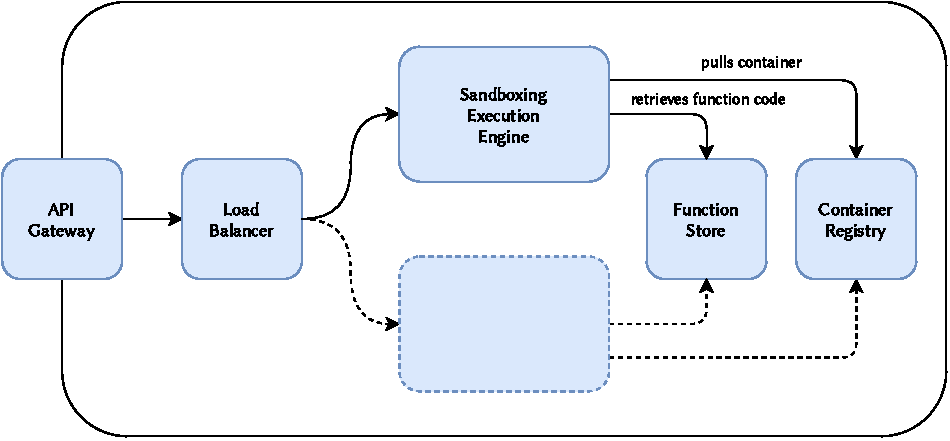
\includegraphics[width=\textwidth]{figures/ServerlessArchitecture.pdf}
    \caption{A generalized serverless architecture based on OpenWhisk, OpenFaaS and OpenLambda.}
    \label{fig:serverless-architecture}
\end{figure}

Based on popular open-source serverless frameworks we can infer what a typical serverless architecture looks like. We use OpenFaaS\footnote{\url{https://www.openfaas.com/}}, Apache OpenWhisk\footnote{\url{https://openwhisk.apache.org/}} and OpenLambda\footnote{\url{https://github.com/open-lambda/open-lambda}} as our basis and sketch this generalized architecture in Figure \ref{fig:serverless-architecture}. The system is exposed through an API Gateway. A user can interact with the system through the gateway and manage (i.e. Create, Read, Update and Delete; or CRUD) functions, set up scheduled triggers or retrieve the results of previous invocations. Once a function is created and an execution request comes in, the load balancer will pick an appropriate host for execution. Each of these runs a sandboxing execution engine, such as Docker or a similar container runtime which runs user workloads in an isolated manner.
Serverless frameworks allow developers to write their functions in a variety of languages; they are almost language-agnostic. Since many popular languages need a runtime, such as \inl{node.js}, Python or a Java \inl{JRE}, these runtimes are baked into container images. In order to execute a function, the container image with the appropriate runtime is pulled from a container registry.
The function's code is retrieved from an internal database. The container is started, the code is injected and made ready for execution. Finally, the function is invoked with the user's parameters and the result returned to the framework, which in turn returns it to the user. Typically, frameworks implement optimizations such as pre-pulling images onto the hosts or keeping started containers around for some time, to avoid the costly first startup on subsequent invocations. Here, we see a discrepancy between the aforementioned ideal of scaling to zero and the real world implementations. If post-invocation, containers are still running but users are no longer billed for them, the incurred cost falls to the platform operator. An ideal framework would be truly scale-to-zero, but there is one issue that prevents them from being so.

\subsection{Cold Start}

In the context of serverless computing, a cold start refers to the invocation of a function, when all of the necessary resources for its execution must be provisioned from scratch. A cold start thus delays the execution of the function itself, by the amount of time it takes for the resources to become ready. This is what we call the cold start latency or cold start time. \citeauthor{Wang2018} have measured the cold start latency at major cloud providers such as Amazon Web Services (AWS) and Google Cloud Platform. The cold start time depends on the allocated memory, from which the CPU allowance is determined, so it is given as well. The median cold start latency for AWS was between 250 ms (1536 MB) and 265 ms (128 MB) and between 110 ms (2048 MB) and 493 ms (128 MB) for Google, both depending on the amount of memory assigned to the instance \cite{Wang2018}.

Cold starts prevent serverless platforms from scaling to zero in practice. If every function would be executed in a newly provisioned container, subsequent invocations of the same function would all incur the cold start debt and would not be performant enough. Thus, typical optimizations are to keep these resources provisioned, such that repeated requests are faster to execute. Apache OpenWhisk, for instance, keeps a function's container paused and ready for reuse for 10 minutes, before removing it entirely. AWS Lambda's cold start policy has been reverse-engineered and the findings indicate that an instance stays alive for a duration of 5 to 7 minutes, during which no cold start will take place \cite{ShilCold2021}.

Cold starts are an issue for latency-sensitive applications, where additional hundreds of milliseconds are unacceptable. \citeauthor{Cui2018} gives examples such as food ordering services, e-commerce sites or social networks, which all have unpredictable bursts of requests at certain points in time. In serverless versions of these applications, these bursts would translate into multiple concurrent cold starts, of which each individual one is slower than a singular, non-concurrent cold start. Thus, the numbers cited above increase significantly with higher concurrency \cite{Mohan2019, Cui2018} -- something that auto-scaling platforms ought to handle particularly well.

\subsection{Serverless Edge Computing}

% https://hal.inria.fr/hal-01677622/file/449571_1_En_15_Chapter.pdf
% They draw attention to the fact, that computational power at the edge is much more finite than the apparently finite level of computing, available at the cloud. "since anoverloaded MEC server significantly degrades user experience and negates theadvantages of MEC". Thus, virtualization and containerization cannot simply be adopted, it is not fine-grained enough. Enter serverless...

Judging by the increasing adoption of the IoT, we are \quot{entering the post-cloud era}, as \citeauthor{Shi2016} write \cite{Shi2016}. The edge computing paradigm promises to be a solution to the massive amounts of data that will be generated at the edge. A wearable body sensor measuring health data for example, can use the wearer's smartphone (edge device) for data processing rather than sending the workload all the way to the cloud. In general, edge devices are machines, that sit between the data source and the cloud. This processing close to the data source has a number of advantages, such as enabling low latency response times as well as working with privacy-sensitive data. This is necessary, since sending all data to the cloud has comparably higher latency and puts more strain on the wide-area network.

One piece of the puzzle towards realizing this paradigm, is serverless edge computing. \citeauthor{Aslanpour2021} lay out the vision for serverless edge computing, of which we highlight two points \cite{Aslanpour2021}.

\begin{itemize}
    \item Due to IoT devices' unpredictable workload, an under- or overprovisioning of static resources such as VMs or containers would be likely. Serverless with its ability to scale to zero (even with aboves caveat) provides more precise provisioning of resources and only incurs cost when used, bringing advantages for operator and user, respectively. Executing serverless workloads in an energy-constrained setting, such as on single-board computers (SBC), this becomes doubly-important.
    \item Serverless computing tends to be used for unpredictable, bursty workloads that require immediate up-scaling. Application architectures for IoT devices are usually event-driven and often unpredictable, making them a perfect fit for serverless.
\end{itemize}

Serverless computing can be the enabler for edge computing. But some of its original design decisions need to be reexamined, as \citeauthor{Nastic2018} point out, due to the

\begin{quote}
    \quot{[...] inherently different nature of Edge infrastructure, for example, in terms of available resources, network, geographical hyper-distribution, very large scale, etc. \cite{Nastic2018}}
\end{quote}

IBM has reacted to these changed requirements and introduced Edge Functions on the IBM Cloud Internet Services \cite{Farid2019}. This offering allows developers to run code closer to the user by deploying functions to their edge network. As a consequence of the resource constraints of edge devices, their offering uses the JavaScript V8 engine and its isolates feature. This is a similar step as moving to a WebAssembly executor, i.e. using a less costly sandboxing mechanism than containers to account for the resource constraints on the edge. Some of their serverless edge computing use cases include »personalized user experiences through conditional routing and originless responses.« The latter means returning responses directly form the edge without going all the way to the cloud \cite{IBM2021}. This leads to another use case: increased API responsiveness through aggregation and caching from multiple cloud-based API endpoints.

\subsection{Serverless Workload}
\label{section:serverless_workload}

Since we aim to redesign the fundamental building block of a serverless framework, namely the underlying container runtime, it is important to examine what the serverless workload looks like. Here, we provide an overview of the research in this area.

\citeauthor{Shahrad2020} have characterized the serverless workload for a large cloud platform: Microsoft Azure. Because of their large number of users, this study can be considered a very good representation of the average workload.
They find that, on average, 81\% of the functions are invoked less than once per minute. However, those accessed more frequently make up 99.6\% of all invocations \cite{Shahrad2020}.
Those frequently accessed functions should thus be kept in memory, to avoid the cold start entirely. The less frequently accessed functions should not be kept in memory, but created, executed and destroyed immediately, in order to save resources. For this to be viable, the cold-start needs to be a cheap operation. In general, the cheaper the cold start, the smaller the amount of time that functions need to be kept in memory.
Customers are only billed for the execution time of the function in FaaS. Operators bear the cost of keeping functions in memory -- or resources warm, more generally. Thus, shorter cold starts reduce costs.

\citeauthor{Shahrad2020} also find that on average, 50\% of functions execute for less than one second.

\begin{quote}
    \quot{The main implication is that the function execution times are at the same order of magnitude as the cold start times reported for major providers. \emph{This makes avoiding and/or optimizing cold starts extremely important for the overall performance of a FaaS offering} \cite{Shahrad2020}.}
\end{quote}

This is corroborated by the cited cold start times of \citeauthor{Wang2018} above.
Because of these findings, the primary goal in this work is that of reducing the cold start latency, to make cold starts a more efficient process in turn enabling reduced keep-alive times. It would then also make the first of a series of function invocations less costly. Moreover, a single more efficient cold start also reduces the cost of concurrent ones -- a particularly time intensive process for Docker containers.
Even in light of a cheap cold start, we still need to make sure that we have a resource-efficient way to keep the function in memory. Consider that the most frequently accessed functions make up an overwhelming share of invocations. This scenario needs to be just as efficient as a cold start and it is unlikely that we achieve a reduction of cold start times to such a degree, that always cold starting these functions will be more efficient than a short keep-alive period.
As \citeauthor{Shahrad2020} point out, there is a fundamental trade-off between using memory to keep functions warm, and forgoing it, but incurring the additional latency of a cold start. Thus, unless we can eliminate the cold start completely, we will need some kind of keep-alive policy. Hence, we note it as a requirement for the implementation and also examine the memory usage of our approach in the evaluation.

\citeauthor{Eismann2021} conducted a study on why companies adopt serverless, for which applications it is best-suited and how they are implemented \cite{Eismann2021}. They analyzed 89 open-source serverless applications, of which 84\% have bursty workloads. Thus, these spikes in demand -- manifested in concurrent requests, in turn causing up-scaling -- ought to be handled well by serverless platforms.
They find 69\% of the applications have a data volume of less than 10 MB. Thus, memory-bound applications are likely not a primary use case. Furthermore, 39\% of the applications have a high traffic intensity, 47\% have a low traffic intensity and 17\% utilize scheduled functions. Thus, the latter combined 64\% represent on-demand scenarios where the platform will experience cold starts, since it is less likely that a warm function exists in those cases. According to the authors, 88\% of the applications make use of Backend-as-a-Service (BaaS) offerings. Storage, databases and messaging services are the most popular ones.
\citeauthor{Leitner2019} carried out a mixed-method study based on grey literature, interviews with serverless practitioners and web-based surveys, to provide an overview of the state of serverless \cite{Leitner2019}. They find that developers who successfully adopted serverless have a different mental model than traditional web-application developers. The former design the application as a composition of standalone, external components, that they have not written themselves. Similar to \citeauthor{Eismann2021}, they also find developers use databases (78\%), API gateways (69\%), logging services (66\%) or IaaS (52\%) in conjunction with their serverless function. They even argue that the real power of FaaS comes from its ability to glue together various existing cloud services.
Typical use cases, according to \citeauthor{Leitner2019}, include processing application data (76\%), like transforming images, performing scheduled jobs (64\%) like notifications or backups or processing monitoring and telemetry data (39\%). With the exception of transforming images, these use cases do not indicate a high CPU usage.

From this we can infer that the majority of functions will make requests to external services, which means those functions will wait for network I/O to complete while the CPU is not actively utilized. More generally, network I/O-bound workloads are a primary type that serverless platforms should be able to handle well. This is further corroborated by the languages typically used to write serverless functions. \citeauthor{Eismann2021} report that the overwhelming share of serverless functions is implemented in interpreted languages such as JavaScript (42\%) and Python (42\%). Data from dashbird.io\footnote{\url{https://dashbird.io/}}, a serverless monitoring tool, underpins the assumption that interpreted languages are dominant. Of their 3000+ users, 76\% use JavaScript, 13\% use Python and 8\% use Java \cite{Rehemaegi2019}. We can see that \inl{node.js} in particular is a highly used engine for serverless. It is best known for its event-driven I/O; less so for being a highly performant computing platform. This, coupled with the fact that interpreted languages make up the majority of serverless languages, has two implications.
One is, that CPU-bound tasks are not the primary serverless use case and can be considered more of a niche. If this were not the case, we would likely see a much higher share of compiled languages. Although, a language like Python can also be extended with performant modules written in C, the dashbird data in particular indicate that \inl{node.js}-level performance is almost always good enough.
The other is, if a new container runtime can be as fast as these interpreted or JIT-compiled languages, we are not suffering from a loss in performance and, if we can be even faster than those, we already have net performance gains to report.

From this research, we might conclude that the current serverless platforms already fulfill these use cases. However, selection bias tells us that the current representation plays towards the strengths of the current approach and would not include use cases which are not working in this environment in the first place.
Indeed, interviewees from the \citeauthor{Leitner2019} study explicitly and repeatedly voiced concerns about building user-facing applications because of the high response times in case of cold starts. The authors concluded that applications requiring high performance or real-time requirements are not suitable to be built on serverless platforms -- at least, not yet. This leads back to the cold start being a real problem that not only incurs resource costs, as explored previously, but, perhaps more importantly, completely inhibits certain use cases.
However, it also shows that the lack of high performance in serverless may be an inhibiting factor as well. With everything in mind, we can neither exclude CPU-bound applications from our focus, nor make them the primary one.

\section{WebAssembly}

For the longest time, JavaScript was the sole client-side language in web browsers. With the rising popularity of the web platform and its growing number of APIs, more and more complex web apps were written, and increasingly in other programming languages. Necessarily, these languages had to treat JavaScript as a target format, like Java bytecode or machine-level assembly, in order to run on the web. Of course, JavaScript was not designed for this and so performance was lacking.

In 2013, a solution to this problem was introduced by engineers at Mozilla, aptly named \inl{asm.js}. It restricts itself to the parts of JavaScript that can be optimized ahead-of-time \cite{Herman2014}. It might be used to compile a C/C++ program to the \inl{asm.js} target format to execute it with a JavaScript runtime faster than the equivalent JavaScript program would be. Benchmarks even showed it to run no more than 1.5$\times$ slower than native code \cite{Zakai2013}.

Finally, WebAssembly (Wasm) was born out of \inl{asm.js} in 2015, with more layers of optimizations. It is a portable and universal binary instruction format for memory-safe, sandboxed execution in a virtual machine.
It is possible to write programs in a variety of languages like C, C++, Rust, AssemblyScript, C\#, Go, Swift and many more, and compile them to Wasm, which finally relieves JavaScript of its role as the universal target format of the web \cite{W3C2020}.

\subsection{Performance}

Compared to \inl{asm.js}, the Wasm binary format is smaller in size (10-20\%) and faster to parse, by an order of magnitude
\cite{Clark2019}. It is 33\% faster than \inl{asm.js} on average \cite{Haas2017}.
\citeauthor{NotSoFast} ran the PolyBenchC benchmark suite to compare Wasm to native code and found that 13 of the 24 benchmarks performed within 10\% of native code \cite{NotSoFast}. However, they argue that the roughly 100 lines of code long benchmarks are not fully representative of typical use cases. They run the SPEC CPU benchmark suite, which are significantly larger POSIX applications. On average, they find Wasm to be slower than native by 1.55$\times$ in Firefox and 1.45$\times$ in Chrome.
% Not representative, if we precompile to native code, but may be relevant if we choose to also evaluate the Wasm runtimes JIT modes
Wasm modules tend to be smaller than native \inl{x86\_64} binaries. On average, Wasm modules have 85\% of the size \cite{Haas2017}.

Serverless functions, by design, are microservices and thus limited in scope. Developers are compelled to write short and efficient functions, since they are billed for the execution time. The PolyBenchC benchmark results are thus likely more representative than the SPEC suite. However, this assumption is good enough and will be an aspect of our evaluation, regardless.
To increase performance and startup time, Wasm modules can be compiled to native code, either by JIT engines at the time of execution, or ahead-of-time by the same JIT engines or AoT compilers. This process produces an artifact specific to the WebAssembly runtime that compiled it. At this point, the universality of the Wasm format is lost. Doing the translation to native code ahead-of-time means the compilation process does not take up time when we need to execute. Consequently, this is an interesting technique to reduce the time it takes to get a WebAssembly module ready for execution.


% The binary format is designed to allow streaming the contents, so that parts of it can be compiled even before the entire module has been transmitted. (but this is actually irrelevant for our OW implementation, since we have the init call first, in which the module is stored in a hashmap, and later the run call, where it is directly read from memory)


\subsection{Security}

Wasm defines two important goals for security.

\begin{quote}
    \quot{(1) protect users from buggy or malicious modules, and (2) provide developers with useful primitives and mitigations for developing safe applications, within the constraints of (1) \cite{W3C2020}.}
\end{quote}

To that end, Wasm uses fault isolation techniques to sandbox the executing module. Interaction with the host environment is only possible through imported functions \cite{W3C2020}. This mechanism represents a \quot{safe foreign function interface} as it can communicate with the outside environment, but not escape the sandbox \cite{Haas2017}. This is an important security feature of Wasm. A module without imports is side-effect free from the host perspective. Even printing \inl{Hello World!} requires importing a \inl{print} function. Similarly, writing to files, network sockets or reading the clock requires imports, which will be discussed more in the next section.

In Wasm, all memory access is confined to a module's \emph{linear memory}. This memory is separate from the code space, which prevents programs from overwriting instructions. Programs can only operate in their own execution environment, but cannot escape. This means Wasm runtimes can safely execute multiple untrusted modules, with their own linear memories, in the same process memory space and without requiring additional isolation \cite{Haas2017}. In particular, »Reading and writing to arbitrary memory locations cannot be expressed in WebAssembly«, because Wasm's memory instructions work with offsets rather than addresses. Furthermore, bounds checking at runtime ensures the instructions write only to the linear memory \cite{Denis2019}.
This is a key aspect that enables Wasm as a lightweight container technology. Only a single instance of a runtime is needed to execute many (e.g. serverless) functions.

In the assembly produced by compiling a C program, the call to a function is expressed as jumping to the address of the function's first instruction. In exploits of such programs, these addresses are often crafted or changed by malicious actors to take control of the program's control flow. In WebAssembly on the other hand, a function is represented as an index in a table, i.e. it introduces an additional level of indirection to express the address. That adds to security, since an arbitrary address to a Wasm function cannot be crafted with Wasm instructions \cite{Denis2019}. And since the program's memory is separate from the function instructions, an attacker also cannot overwrite them.
Wasm thus features control flow integrity, because it enforces structured control flow. Jump targets and other properties are validated in a single pass before a module is instantiated. In particular, validation prevents jumps from targeting arbitrary locations. This validation must happen, according to the Wasm specification, before a module is executed by a runtime \cite{Haas2017}.

\citeauthor{Lehmann2020} provide a critique of WebAssembly's binary security \cite{Lehmann2020}. Many mitigations that have made \inl{x86} binaries safer, are not present in WebAssembly. According to them, this »re-enables several formerly defeated attacks«. Some of the important points include the following:

\begin{itemize}
    \item Because all data such as constants, the call stack and the heap are in Wasm's linear memory, and any offset from up to the current memory's size is valid, overflows can corrupt any of these. In native binaries on the other hand, these are separate sections protected through unmapped pages, such that an overflow would result in program termination.
    \item Buffer overflows on the stack or heap, as well as stack overflows themselves can be used to obtain a write primitive. Native binaries prevent stack overflows from corrupting data with stack canaries \cite{Cowan98}.
    \item There is no address space layout randomization in Wasm, which would make exploits harder to execute, since a pointer to the stack or heap needs to be obtained first.
    \item Wasm programs ship with their own memory allocator, whose size is important since Wasm is often transmitted over the network. Smaller implementations of allocators such as \inl{emmalloc} re-enable attacks against allocator metadata.
\end{itemize}

\citeauthor{Wingo2020} points out that writing software in memory-safe languages, such as Rust or garbage-collected ones, is »a comprehensive fix to this class of bug« \cite{Wingo2020}. C and C++, on the other hand, are not memory-safe languages. Thus, while the criticism above is valid for programs written in memory-unsafe languages, it does not apply to memory-safe programs. But there is more subtlety to it, since, for example, Rust programs may also link to C programs, which are always considered memory unsafe by the compiler. They can also include blocks of \inl{unsafe} code, where developers can generally use operations that the compiler cannot prove to be safe like dereferencing raw pointers. In both cases the compiler cannot guarantee the program to be memory-safe. Whether WebAssembly should include mitigations for issues, that certain classes of programs do not need, or whether they have to be added to the appropriate compiler toolchains, remains to be discussed.

The presented vulnerabilities apply to a Wasm program itself, but do not enable compromising the host system. Thus, to the best of our knowledge, the current research does not show breakage of WebAssembly's isolation. With both performance and host security under its belt, as well as being a portable and universal target format, Wasm turns out to be useful not just in the browser, but also outside of it.

% We present MS-Wasm, an extension to Wasm that bridges thisgap by allowing developers to capture low-level C/C++ memorysemantics such as pointers and memory allocation in Wasm, at com-pile time. At deployment time, Wasm compilers and JITs can lever-age these added semantics to enforce different models of memorysafety depending on user preferences and what hardware is avail-able on the target platform.
% https://cseweb.ucsd.edu/~dstefan/pubs/disselkoen:2019:ms-wasm.pdf

\subsection{System Interface}

Wasm targets an abstract machine, so it needs an interface to the system. In the web browser, that works by calling into the browser through JavaScript glue code. Outside of it, a new solution was needed: The WebAssembly System Interface (WASI). This interface was designed with Wasm's goals -- portability and security -- in mind.
WASI is binary-compatible, which means that Wasm binaries are portable between different concrete systems like Linux and Windows, but also browsers. The Wasm runtimes effectively implement that interface and translate it to the underlying concrete system.
WASI also innovates in security, over the classic coarse-grained access control. It specifies a fine-grained capability-based security model, that consists of two parts. First, WASI makes use of the aforementioned import mechanism of Wasm, to adhere to its security model. The Wasm module cannot directly call an OS system call due to sandboxing, but imports equivalent WASI functions instead \cite{Clark2019}. For instance, a module that wants to open a file needs import statements like these, given in the WebAssembly text format:

\begin{minted}{wat}
(import "wasi_snapshot_preview1" "fd_read" (func (;5;) (type 8)))
(import "wasi_snapshot_preview1" "path_open" (func (;7;) (type 22)))
\end{minted}

The runtime needs to supply those imports, or the module cannot run. In effect, the runtime and module need to be in consensus about which functions can be accessed. In a serverless context for example, the cloud provider could grant or refuse access to certain functions, enabling security policies on a per-function basis. However, even that is not fine-grained enough. The cloud provider might only want to allow serverless functions to cache some data temporarily in the \inl{/tmp/} directory, but not allow opening \inl{/etc/passwd}. This is where WASI takes ideas from capability-based security.

In order to open a file, the module needs to call functions accessing the file, like \inl{fd\_read}, with a preopened file descriptor \cite{Clark2019}. The Wasm module then has the \emph{capability} to access \emph{that} file, but not others. The file can be opened by the runtime itself, or the program that embeds the runtime. They store that file descriptor in a special WASI module which the runtime -- similar to a dynamic linker -- links to the Wasm module from where it imports the functions. Again, this gives the embedder, e.g. a cloud provider, the chance to customize the exact capabilities on a fine-grained level.

\subsection{Execution}

Just like Java Bytecode needs a JVM, Wasm needs a runtime as well. Since WebAssembly itself is just a specification, we need a concrete implementation to execute a module. There are many implementations available, the most used ones likely being those in the major browser JavaScript engines. However, since we do not need support for JavaScript in this work, we choose to use standalone runtimes. The absence of JavaScript support may also provide a smaller runtime. Those come with different execution engines and goals. Wasm can be interpreted, just-in-time compiled or compiled to native code, ahead-of-time. All of these have different properties in terms of their cold-start latency as well as their runtime performance. We discuss and select concrete runtimes in Chapter \ref{chapter:design}.

% Potential further discussions:
% \begin{itemize}
%     \item Compare with docker in terms of sandboxing, security, system interface, performance, resource cost
%     \item To what degree can we control access to resources in Wasm, i.e. limit memory or CPU shares -- equivalents of docker's \inl{--memory} and \inl{--cpu-shares} options?
%     \item Linux Containers in general, Docker, i.e. define »container« and »container runtime«. Why are containers slow to start?
% \end{itemize}